\documentclass[10pt]{amsart}
\usepackage{amsmath}
\usepackage{graphicx}
\newtheorem{theorem}{Theorem}
\newtheorem{proposition}[theorem]{Proposition}
\newtheorem{corollary}[theorem]{Corollary}
\newtheorem{lemma}[theorem]{Lemma}
\usepackage[margin=2.5 cm]{geometry}
\usepackage{parskip}
\usepackage{mathtools}
\usepackage{multicol}

\renewcommand{\labelenumi}{(\alph{enumi})}
\begin{document}
\centerline{\bf Math Camp - Homework 6 Solutions}


\section{Linear Algebra}


\textbf{Question 1}: Determine  whether the following matrices are invertible. Justify your answer. (Note: You do not need to find the inverse, just say whether it exists.)

\begin{multicols}{3}
	\begin{enumerate}
		\item $\mathbf{A} = \left[\begin{matrix*}[r]
		1 & 9 & 6 \\
		3 & 10 & -1 \\
		8 & 38 & 10
		\end{matrix*}\right]$
		
		\item $\mathbf{B} = \left[\begin{matrix*}[r]
		8 & -2 & 4 & 10 \\
		0 & 0 & 1 & -1 \\
		-9 & 8 & 0 & 0 \\
		1 & 0 & 0 & 0
		\end{matrix*}\right]$
		
		\item $\mathbf{C} = \left[\begin{matrix*}[r]
		0 & 1 \\
		0 & 0
		\end{matrix*}\right]$
	\end{enumerate}
\end{multicols}

\textbf{Solution}

There are several ways that you could go about showing that a matrix is invertible without actually finding its inverse. The first way is to investigate whether the rows and columns are linearly independent. 

Recall that for a matrix to be invertible, both the row and column vectors need to be linearly independent. That is, suppose 
\begin{align*}
\mathbf{S} = \left[\begin{matrix*}[r]
\mathbf{s}_1 \\
\mathbf{s}_2 \\
\vdots \\
\mathbf{s}_n \\
\end{matrix*}\right]
\end{align*} where $\mathbf{s}_i$ are row vectors. Then $\mathbf{S}$ is invertible if and only if $\mathbf{s}_1, \mathbf{s}_2, \dots, \mathbf{s}_n$ are linearly independent.  To check for linear independence, it  must be the case that the only solution to the equation
\begin{align*}
c_1 \mathbf{s}_1 + c_2 \mathbf{s}_2 + \dots + c_n \mathbf{s}_n =\mathbf{ 0}
\end{align*}
is $c_1 = c_2 = \dots = c_n = 0$. We can use these facts to check whether the given matrices are invertible (without actually calculating any inverses). 

Another way is to check whether the determinant of the matrix is 0. Recall that a matrix is invertible if and only if its determinant is nonzero. 

\begin{enumerate}
	\item Let $\mathbf{a}_1, \mathbf{a}_2, \mathbf{a}_3$ denote the row vectors of $\mathbf{A}$. The third row is a linear combination of the first two rows, so the matrix is not invertible. In particular, let $c_1 = 2$, $c_2 = 2$, and $c_3 = -1$. Then we can verify:
	\begin{align*}
	c_1 \mathbf{a}_1 + c_2 \mathbf{a}_2 + c_3 \mathbf{a}_3 &= 2 \left[\begin{matrix}
	1 \\9 \\6
	\end{matrix}\right] + 2 \left[\begin{matrix*}[r]
	3 \\ 10 \\ -1
	\end{matrix*}\right] - \left[\begin{matrix*}[r]
	8 \\ 38 \\ 10
	\end{matrix*}\right] \\
	&= \left[\begin{matrix*}[r]
	2 \\ 18 \\ 12
	\end{matrix*} \right] + \left[\begin{matrix*}[r]
	6 \\\ 20 \\ -2
	\end{matrix*}\right] - \left[\begin{matrix*}[r]
	8 \\ 38 \\ 10
	\end{matrix*}\right] = \left[\begin{matrix*}[r]
	0\\0\\0
	\end{matrix*}\right]
	\end{align*}
	Because we could find nonzero coefficients $c_1$, $c_2$, and $c_3$ that solve the system of equations, the rows are linearly dependent and $\mathbf{A}$ is not invertible. 
	
	\item Let's put this matrix into \texttt{R} and find its determinant. 
	\begin{verbatim}
	> B = matrix(c(8, -2, 4, 10, 
						               0, 0, 1, -1, 
						               -9, 8, 0, 0, 
						               1, 0, 0, 0), nrow=4, ncol=4, byrow=T)
	> det(B)
	[1] 112
	\end{verbatim}
	Since the determinant of $\mathbf{B}$ is $|\mathbf{B}| = 112 \ne 0$, the matrix is invertible. 
	
	\item Again, let's look at the determinant. Recall from the last homework (or from the definition of determinants) that for a $2\times2$ matrix $\mathbf{M} = \left[\begin{matrix}m_{11} & m_{12} \\ m_{21} & m_{22}\end{matrix}\right]$, the determinant is $|\mathbf{M}| = m_{11} m_{22} - m_{12}m_{21}$. Applying this definition, we have $|\mathbf{C}| = 0\cdot0 - 1\cdot0 = 0$. Thus, $\mathbf{C}$ is singular. 
\end{enumerate}


\bigskip


\textbf{Question 2:} Recall from lecture that, given an $n\times n$ matrix $\mathbf{A}$, if there exists a vector $\mathbf{x}$ and scalar $\lambda$ such that 
\begin{eqnarray*}
	\mathbf{A}\mathbf{x} = \lambda \mathbf{x}
\end{eqnarray*}
then we say that $\mathbf{x}$ is an eigenvector and $\lambda$ is an eigenvalue for $\mathbf{A}$. 

Now consider the matrix
\begin{align*}
M &= \left[\begin{matrix*}[r]
3 & -1 & 1 \\
1 & 1 & 1 \\
1 & -1 & -3 \\
\end{matrix*}\right]
\end{align*}
along with the eigenvalues $\lambda_1 = -3$, $\lambda_2 = 2$, and $\lambda_3 = 2$ and eigenvalues 
\begin{align*}
\mathbf{x}_1 = \left[\begin{matrix*}[r]
-1 \\ -1 \\ 5
\end{matrix*}\right]   & &
\mathbf{x}_2 = \mathbf{x}_3 = \left[\begin{matrix*}[r]
1 \\ 1\\ 0
\end{matrix*}\right]
\end{align*}

\begin{enumerate}
	\item For each eigenvalue/vector pair $i$, show that $\mathbf{M} \mathbf{x}_i = \lambda_i \mathbf{x}_i$. 
	
	\item One way to calculate the eigenvalues of $\mathbf{A}$ is to find the values of $\lambda$ that solve the equation $$\det(\mathbf{A} - \lambda I) = 0,$$ where $I$ is the identity matrix. Show that this fact holds for $\mathbf{M}$ given above. 
\end{enumerate}

\textbf{Solution} 
\begin{enumerate}
	\item We can straightforwardly verify for $\mathbf{x}_1$:
	\begin{align*}
		\mathbf{M} \mathbf{x}_1 &=  \left[\begin{matrix*}[r]
		3 & -1 & 1 \\
		1 & 1 & 1 \\
		1 & -1 & -3 \\
		\end{matrix*}\right] %
		\left[\begin{matrix*}[r]
		-1 \\ -1 \\ 5
		\end{matrix*}\right] \\
		&= \left[\begin{matrix*}[r]
		-3 +1 +5 \\
		-1 -1 +5 \\
		-1 + 1 -5
		\end{matrix*}\right] \\
		&= \left[\begin{matrix*}[r]
			3 \\ 3 \\ -15
		\end{matrix*}\right] = -3 \mathbf{x}_1 = \lambda_1 \mathbf{x}_1
	\end{align*}
	
	and for $\mathbf{x}_2$:
	
	\begin{align*}
		\mathbf{M} \mathbf{x}_1 &=  \left[\begin{matrix*}[r]
		3 & -1 & 1 \\
		1 & 1 & 1 \\
		1 & -1 & -3 \\
		\end{matrix*}\right] %
		\left[\begin{matrix*}[r]
		1 \\ 1 \\ 0
		\end{matrix*}\right] \\
		&= \left[\begin{matrix*}[r]
		3 -1 + 0 \\
		1 +1 + 0  \\
		1 - 1 + 0
		\end{matrix*}\right] \\
		&= \left[\begin{matrix*}[r]
		2 \\ 2 \\ 0
		\end{matrix*}\right] = 2\mathbf{x}_2 = \lambda_2\mathbf{x}_2
	\end{align*}
	Since the third eigenvalue and eigenvector are the same as the second, we're finished. 
	
	\item Let's first write out $\mathbf{M} - \lambda \mathbf{I}$:
	\begin{align*}
		\mathbf{M} - \lambda \mathbf{I} &= \left[\begin{matrix*}[r]
		3 & -1 & 1 \\
		1 & 1 & 1 \\
		1 & -1 & -3 \\
		\end{matrix*}\right] - \left[\begin{matrix*}[r]
		\lambda & 0 & 0 \\ 0 & \lambda & 0 \\ 0 & 0 & \lambda
		\end{matrix*}\right] \\
		&= \left[\begin{matrix*}[r]
		3 - \lambda & -1 & 1 \\
		1 & 1  - \lambda & 1 \\
		1 & -1 & -3 - \lambda \\
		\end{matrix*}\right]
	\end{align*}
	Now, we can find the determinant of this  new matrix and set it equal to 0. This is called the characteristic polynomial of $\mathbf{M}$:
	\begin{align*}
		0 &= (3 - \lambda)(1 - \lambda)(-3-\lambda) + (-1)(1)(1) + (1)(1)(-1)  - (1)(1-\lambda)(1) - (-1)(1)(-3-\lambda) - (3-\lambda)(1)(-1) \\
		0 &= (3 - \lambda)(1 - \lambda)(-3-\lambda)  -2 - (1-\lambda) + (-3 - \lambda) + (3 - \lambda)
	\end{align*}
	If we didn't already know the eigenvalues, we could solve for the roots of this polynomial to find them. In this case, we can simply plug in the given values $\lambda = -3$ and $\lambda = 2$  and verify that they solve the equation.
\end{enumerate}



\section{Calculus with Many Variables}

\textit{Notation note:} It's worthwhile to familiarize yourself with two common ways of denoting partial derivatives. Given some function $f(x,y)$, 
\begin{equation*}\frac{\partial f}{\partial x} = f_x \qquad \frac{\partial f}{\partial y} = f_y \qquad \frac{\partial^2 f}{\partial x^2} = f_{xx} \qquad \frac{\partial}{\partial y} \frac{\partial f}{\partial x} = \frac{\partial^2 f}{\partial y \partial x} = f_{xy} \qquad \frac{\partial}{\partial x} \frac{\partial f}{\partial y} = \frac{\partial^2 f}{\partial x \partial y} = f_{yx} \qquad \frac{\partial^2 f}{\partial y^2} = f_{yy}\end{equation*}

You're free to use either, but {\it please} use them -- they are essential. Do not leave your calculations unlabeled.

\textbf{Question 3:} Find all of the first partial derivatives of each function.

\begin{enumerate}
\item $f(x,y) = 3x - 2y^4$

\item $f(x,y) = x^5 + 3x^3y^2 + 3xy^4$

\item $g(x,y) = xe^{3y}$

\item $k(x,y) = \frac{x-y}{x+y}$

\item $f(x,y,z) = \log(x+2y+3z)$

\item $h(x,y,z) = x^2 e^{yz}$
\end{enumerate}

\textbf{\textit{Solutions}}
\begin{enumerate}
\item The partial derivatives here involve straightforward power rule. As you do these partial derivatives, get used to seeing all other variables that you're not interested in as constants. It will become more natural over time.
$$\frac{\partial f}{\partial x} = 3 \qquad \frac{\partial f}{\partial y} = -8y^3$$

\item More power rule.
$$\frac{\partial f}{\partial x} = 5x^4 + 9x^2y^2 + 3y^4 \qquad \frac{\partial f}{\partial y} = 6x^3y+12xy^3$$

\item Now, we have to start dealing with chain rule. Note that even though there is technically a product involving $x$ and $y$ here, at no point does either variable show up in both parts of the product. As such, we don't need product rule.

The partial derivative with respect to $x$ is straightforward. The function is linear with respect to $x$, so the partial derivative is $e^{3y}$.

The partial derivative with respect to $y$ is a bit more complicated.
$$\frac{\partial g}{\partial y} = xe^{3y} \cdot \frac{\partial}{\partial y}(3y) = xe^{3y} \cdot 3 = 3xe^{3y}$$

\item We require the use of quotient rule here. (Or as we showed in a previous homework, you can rewrite this as a product.) Recall that the quotient rule for some generic $h(x) = \frac{f(x)}{g(x)}$ is
$$h'(x) = \frac{f'(x)g(x)-f(x)g'(x)}{(g(x))^2}$$

So, we can apply this formula to derive the function with respect to each variable to get:
\begin{align*}
\frac{\partial k}{\partial x} &= \frac{(\frac{\partial}{\partial x} (x-y)) (x+y) - (x-y) (\frac{\partial}{\partial x} (x+y))}{(x+y)^2} \\
&= \frac{(1)(x+y) - (x-y)(1)}{(x+y)^2} \\
&= \frac{x+y-x+y}{(x+y)^2} \\
&= \frac{2y}{(x+y)^2}
\end{align*}
\begin{align*}
\frac{\partial k}{\partial y} &= \frac{(\frac{\partial}{\partial y} (x-y)) (x+y) - (x-y) (\frac{\partial}{\partial y} (x+y))}{(x+y)^2} \\
&= \frac{(-1)(x+y) - (x-y)(1)}{(x+y)^2} \\
&= \frac{-x-y-x+y}{(x+y)^2} \\
&= -\frac{2x}{(x+y)^2}
\end{align*}


\item This requires relatively straightforward chain rule.
$$\frac{\partial f}{\partial x} = \frac{1}{x+2y+3z} \cdot \frac{\partial}{\partial x}(x+2y+3z) =
\frac{1}{x+2y+3z}(1) = \frac{1}{x+2y+3z}$$
$$\frac{\partial f}{\partial y} = \frac{1}{x+2y+3z} \cdot \frac{\partial}{\partial y}(x+2y+3z) =
\frac{1}{x+2y+3z}(2) = \frac{2}{x+2y+3z}$$
$$\frac{\partial f}{\partial z} = \frac{1}{x+2y+3z} \cdot \frac{\partial}{\partial z}(x+2y+3z) =
\frac{1}{x+2y+3z}(3) = \frac{3}{x+2y+3z}$$

\item This requires some chain rule, as well.
$$\frac{\partial h}{\partial x} = 2x^{(2-1)}e^{yz} = 2xe^{yz}$$
$$\frac{\partial h}{\partial y} = x^2 e^{yz} \cdot \frac{\partial}{\partial y}(yz) = x^2 e^{yz} \cdot z = x^2 z e^{yz}$$
$$\frac{\partial h}{\partial z} = x^2 e^{yz} \cdot \frac{\partial}{\partial z}(yz) = x^2 e^{yz} \cdot y = x^2 y e^{yz}$$

\end{enumerate}
\medskip

\textbf{Question 4:} Find the gradient $\nabla f$ of the following functions and evaluate them at the given points.
\begin{enumerate}
\item $f(x,y) = \sqrt{x^2 + y^2}$, \quad $(x,y) = (3,4)$
\item $f(x,y,z) = (x+z)e^{x-y}$, \quad $(x,y,z) = (1,1,1)$
\end{enumerate}

\textit{\textbf{Solutions}}
\begin{enumerate}
\item Let's first rewrite the function so that it is easier to differentiate.
$$f(x,y) = \sqrt{x^2 + y^2} = (x^2 + y^2)^{1/2}$$

Now, taking the partial derivatives with respect to $x$ and $y$ comes more naturally.

\begin{align*}
\frac{\partial f}{\partial x} &= \frac{1}{2}(x^2 + y^2)^{-1/2} \cdot \frac{\partial}{\partial x} (x^2 + y^2) \\
&= \frac{1}{2}(x^2 + y^2)^{-1/2} \cdot (2x) \\
&= x (x^2 + y^2)^{-1/2} \\
&= \frac{x}{\sqrt{x^2 + y^2}}
\end{align*}
\begin{align*}
\frac{\partial f}{\partial y} &= \frac{1}{2}(x^2 + y^2)^{-1/2} \cdot \frac{\partial}{\partial y} (x^2 + y^2) \\
&= \frac{1}{2}(x^2 + y^2)^{-1/2} \cdot (2y) \\
&= y (x^2 + y^2)^{-1/2} \\
&= \frac{y}{\sqrt{x^2 + y^2}}
\end{align*}

So, the gradient of this function is
\medskip
\begin{equation*}
\nabla f(x,y) = \left(\frac{x}{\sqrt{x^2 + y^2}}, \frac{y}{\sqrt{x^2 + y^2}}\right)
\end{equation*}

And if we evaluate it at the given point, we get
\medskip
\begin{equation*}
\nabla f(3,4) = \left(\frac{3}{\sqrt{3^2 + 4^2}}, \frac{4}{\sqrt{3^2 + 4^2}}\right) = \left(\frac{3}{\sqrt{9 + 16}}, \frac{4}{\sqrt{9 + 16}}\right) = \left(\frac{3}{\sqrt{25}}, \frac{4}{\sqrt{25}}\right) = \left(\frac{3}{5}, \frac{4}{5}\right) 
\end{equation*}

\item This question is slightly more involved; the partial derivative with respect to $x$ will require product rule since $x$ appears in both factors of the product. Recall that the product rule for a generic $h(x) = j(x)k(x)$ is $h'(x) = f'(x)g(x) + f(x)g'(x)$. The partial derivative with respect to $y$ will require chain rule.
\medskip
\begin{align*}
\frac{\partial f}{\partial x} &= \left(\frac{\partial}{\partial x}(x+z)\right) e^{x-y} + (x+z) \left(\frac{\partial}{\partial x} e^{x-y}\right)\\
&= (1) \cdot e^{x-y} + (x+z) \cdot e^{x-y}\\
&= e^{x-y} + (x+z) \cdot e^{x-y}\\
&= e^{x-y} (x+z+1)
\end{align*}

(The partial derivative above technically requires chain rule where you take the derivative of $x-y$ with respect to $x$, but that's just 1, so we omit that work here.)
\medskip
\begin{align*}
\frac{\partial f}{\partial y} &= (x+z)\cdot e^{x-y} \cdot \left(\frac{\partial}{\partial y} (x-y)\right)\\
&= (x+z) \cdot e^{x-y} \cdot (-1)\\
&= -e^{x-y}(x+z)
\end{align*}
\end{enumerate}

\begin{align*}
\frac{\partial f}{\partial z} &= \frac{\partial}{\partial z} (xe^{x-y} + ze^{x-y}) \\
&= \frac{\partial}{\partial z} (xe^{x-y}) + \frac{\partial}{\partial z} (ze^{x-y}) \\
&= 0 + e^{x-y}\\
&= e^{x-y}
\end{align*}

The gradient of this function, which we can also write as a vertical vector, is

$$\nabla f(x,y,z) = \left[\begin{array}{r} e^{x-y} (x+z+1) \\ -e^{x-y}(x+z) \\ e^{x-y}\end{array}\right]$$

When we evaluate the gradient at the given value, we obtain

$$\nabla f(1,1,1) = \left[\begin{array}{c} e^{1-1} (1+1+1) \\ -e^{1-1}(1+1) \\ e^{1-1}\end{array}\right] = \left[\begin{array}{r} e^0 (3) \\ -e^0 (2) \\ e^0) \end{array}\right] = \left[\begin{array}{r} 1 \cdot 3 \\ -1 \cdot 2 \\ 1\end{array}\right] = \left[\begin{array}{r} 3 \\ -2 \\ 1 \end{array}\right]$$

\medskip

\noindent \textbf{Question 5:} Suppose we were interested in learning about how years of schooling affect the probability that a person turns out to vote. To simplify things, let's say we're trying to predict whether one individual voted. We did some preliminary work on this in Problem Set 2, Question 7, but suppose we showed a colleague our model from this problem and they complained. ``What a lame model," our colleague said, ``You definitely have to include an intercept term." So in this problem we'll follow our colleague's advice and do just that.\\

Let $Y$ be our single observation of the dependent variable (whether or not a person turned out to vote) and $X_1$ be our single observation of an independent variable, $education$, the number of years of schooling for this individual. Now though, we're also gong to include an intercept term, $\beta_0$ in our model along with $\beta_1$ a coefficient that's associated with $X_1$. 

This produces the following model for which we want to find the values of both $\beta_0$ and $\beta_1$ that minimize the sum of square errors. 

\bigskip
\begin{eqnarray*}
Y&=& \beta_0 + \beta_1 X_1 + \epsilon\\
 \end{eqnarray*}
 
 where $\epsilon$ is an error term.
 
 Use the method of least squares to solve for the values of $\beta_0, \beta_1$ that minimizes the sum of squared errors in the our data. Using the tools of multivariate minimization we've been practicing, find the values of $\beta_0$ and $\beta_1$ that minimize this quantity.
 
\textbf{Solutions}
 \begin{eqnarray*}
 Y&=& \beta_0 + \beta_1 X_1 + \epsilon\\
 Y - (\beta_0 + \beta_1 X_1) &=& \epsilon\\
 (Y - (\beta_0 + \beta_1 X_1) )^2 &=& \epsilon^2
 \end{eqnarray*}
 
 \begin{eqnarray*}
 f(\beta_0, \beta_1 | x_i, y_i) &=& (Y - \beta_0 - \beta_1 X_1 )^2\\
% &=& Y^2 - Y\beta_0 + Y \beta_1 X_1 -\beta_0Y + \beta_0^2 - \beta_0\beta_1 X_1 + Y\beta_1X_1 - \beta_0 \beta_1 X_1 - (\beta_1 X_1)^2\\
\dfrac{\partial{ f(\beta_0, \beta_1 | x_i, y_i)}}{\partial \beta_0} &=& -2(Y - \beta_0 - \beta_1X_1)\\
&=& -2Y + 2\beta_0 + 2\beta_1 X_1\\
0 &=& 2Y - 2\beta_0 - 2\beta_1 X_1\\
\hat \beta_0 &=& Y - \beta_1X_1\\
\dfrac{\partial{ f(\beta_0, \beta_1 | x_i, y_i)}}{\partial \beta_1} &=& -2 X_1( Y - \beta_0 - \beta_1 X_1)\\
&=&  -2YX_1 + 2\beta_0 X_1 + 2\beta_1 X_1^2\\
0 &=& 2YX_1 - 2\beta_0 X_1 - 2\beta_1 X_1^2\\
\beta_1 X_1^2 &=& YX_1 - \beta_0 X_1\\
\end{eqnarray*}
We then sub in $\hat \beta_0$ for $\beta_0$ and continue:
\begin{eqnarray*}
\beta_1 X_1^2 &=& YX_1 - (Y - \beta_1X_1)X_1\\
\beta_1 X_1^2 &=& YX_1 - YX_1 + \beta_1 X_1^2\\
\beta_1 X_1^2  &=& \beta_1 X_1^2\\
\beta_1 X_1^2  - \beta_1 X_1^2 &=& 0\\
0 &=& 0\\
 \end{eqnarray*}
 
 So, what's going on? Why can't we find a solution for $ \hat \beta_1$?
 
 The problem is that we are trying to use two parameters to describe a single observation of data. This is a case of a problem that occurs when solving systems of equations known as ``underdetermination" (i.e., we have two unknown parameters, $\beta_0$ and $\beta_1$, but only one equation with which to estimate them).\\
 
 \begin{verbatim}http://en.wikipedia.org/wiki/Underdetermined_system\end{verbatim}
 
 The intuition behind this problem is that, given our data, we don't have enough information to uniquely identify two parameters. With one observation we could minimize the squared error by \textit{either} \textbf{1)} fitting the point exactly with our intercept term, $\beta_0$,  \textbf{2)} fitting the point exactly with the parameter on education $\beta_1$ or \textbf{3)} fitting the point with some linear combination of values for $\beta_0$ and $\beta_1$. Assuming this individual voted (y=1) and had 10 years of education (x=10), the line in Figure 1 shows the all the pairs of parameter estimates that would minimize the squared error with the two edge cases as end points (i.e., explain entirely with the intercept term or with the parameter attached to education) and a number of combinations of parameter values that also work in between (e.g., $\beta_0 = .5$ and $\beta_1=.05$).  
 
 \begin{figure}[!ht]
\centering
\caption{Parameter Solutions that Minimize Squared Error in Problem 5}
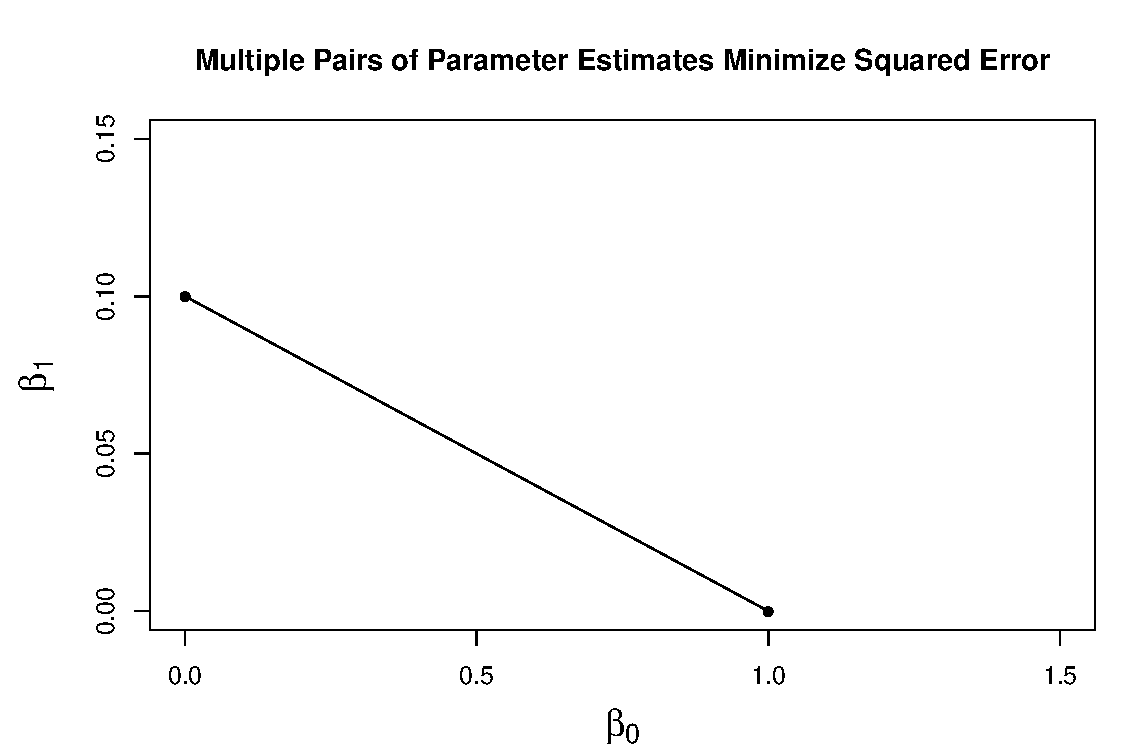
\includegraphics[height=3.5in, width=4.5in]{hw6answers.pdf}
\end{figure}
 
 Since we have so many different combinations of parameter values that accomplish our goal, to minimize the squared error, equally well, no unique solution exists for this parameter vector. When this occurs we say our model is not identified. 
   
If we start to get more observations than parameters we want to estimate (i.e., we have an overdetermined system of equations), this answer will change and we'll get unique solutions for each.\\
 
 \textbf{A couple notes}:
 
 \textbf{Note 1}\\
This problem illustrates, in a very simple manner, one symptom of underdetermination: perfect multicollinearity. Because we have a linearly dependent matrix X'X, it means we can't invert it in order to estimate ordinary least squares (i.e., $ \hat \beta = (X'X)^{-1}X'Y$). 
 
 \begin{eqnarray*}
X &=& \begin{bmatrix} 1 & X_1 \end{bmatrix}\\
X'X &=& \begin{bmatrix} 1 \\
					X_1 \end{bmatrix} \begin{bmatrix} 1 & X_1 \end{bmatrix}\\
	&=& \begin{bmatrix} 1 & X_1 \\
		X_1 & X_1^2 \end{bmatrix}
\end{eqnarray*}
\\
Where we can show linear dependence by multiplying the first row in the matrix by $X_1$ to get an exact copy of the second row. This is an issue we will continue to deal with in 450A. We'll see that perfect multicollinearity can also occur even when we have more observations than variables, if we can write some variables as a linear combination of other variables. 

\textbf{Note 2}\\
If you got values for $\hat \beta_0$ and $\hat \beta_1$ on this problem you did something wrong (e.g., assumed more than 1 observation, made an algebra mistake).  

%\end{enumerate}

\end{document}